%%
% This is an Overleaf template for presentations
% using the TUM Corporate Desing https://www.tum.de/cd
%
% For further details on how to use the template, take a look at our
% GitLab repository and browse through our test documents
% https://gitlab.lrz.de/latex4ei/tum-templates.
%
% The tumbeamer class is based on the beamer class.
% If you need further customization please consult the beamer class guide
% https://ctan.org/pkg/beamer.
% Additional class options are passed down to the base class.
%
% If you encounter any bugs or undesired behaviour, please raise an issue
% in our GitLab repository
% https://gitlab.lrz.de/latex4ei/tum-templates/issues
% and provide a description and minimal working example of your problem.
%%

\documentclass[
  german,            % define the document language (english, german)
  aspectratio=169,    % define the aspect ratio (169, 43)
  % handout=2on1,       % create handout with multiple slides (2on1, 4on1)
  % partpage=false,     % insert page at beginning of parts (true, false)
  % sectionpage=true,   % insert page at beginning of sections (true, false)
]{tumbeamer}


% load additional packages
\usepackage{booktabs}
\usepackage{graphicx}
\usepackage{tikz}
\usepackage{url}
\usepackage{pgfplots}
\usepackage{hyperref}
\usepackage{pmboxdraw}
\usepackage{float}
\usepackage{babel}[ngerman]
\usepackage{csquotes}[autostyle]
\usepackage[useregional]{datetime2}
\usepackage{listings}
\usepackage{xurl}
\usepackage{enumerate}
\usepackage{circuitikz}
\usepackage{csquotes}
\usepackage{tikz-timing}
\usepackage{colortbl}

%\usepackage{minted}
%\usemintedstyle{borland}
\usetikzlibrary{patterns}
\pgfplotsset{compat=1.18}

% tikz
\usetikzlibrary{overlay-beamer-styles}
\usetikzlibrary{arrows,backgrounds,positioning,shapes,,patterns,patterns.meta,matrix,arrows,shapes.geometric}
\usetikzlibrary{matrix, fit}
\usetikzlibrary{automata}
% requires circuitikz >= 1.1.0
% for distros with older distributions, install TeX Live manually
% instead of using your package manager
% see: https://tug.org/texlive/quickinstall.html
\ctikzset{logic ports=european}

% minted

\lstset {
    frame=single,
    tabsize=4,
    breaklines=true,
    xleftmargin=5pt,
    xrightmargin=5pt,
    basicstyle=\ttfamily\footnotesize,
    %language=[RISC-V]Assembler,
}

\hypersetup { 
  colorlinks=true,
  urlcolor=blue,
  filecolor=black,
  linkcolor=black
}

% tikz  
\usetikzlibrary{fit}

% image path
\graphicspath{ {../resources/} }

% presentation metadata
\title{Übung 09: RISC-V Multicycle Prozessor}

\subtitle{Einführung in die Rechnerarchitektur}

\author{\theAuthorName}

\institute{\theGroupName\\\theSchoolName\\\theUniversityName}
\date{16. -- \DTMdisplaydate{2024}{12}{22}{-1}}

\footline{\insertauthor~|~\insertshorttitle~|~\insertshortdate}


% macro to configure the style of the presentation
\TUMbeamersetup{
  title page = TUM tower,         % style of the title page
  part page = TUM toc,            % style of part pages
  section page = TUM toc,         % style of section pages
  content page = TUM more space,  % style of normal content pages
  tower scale = 1.0,              % scaling factor of TUM tower (if used)
  headline = TUM threeliner,      % which variation of headline to use
  footline = TUM default,         % which variation of footline to use
  % configure on which pages headlines and footlines should be printed
  headline on = {title page},
  footline on = {every page, title page=false},
}


% available frame styles for title page, part page, and section page:
% TUM default, TUM tower, TUM centered,
% TUM blue default, TUM blue tower, TUM blue centered,
% TUM shaded default, TUM shaded tower, TUM shaded centered,
% TUM flags
%
% additional frame styles for part page and section page:
% TUM toc
%
% available frame styles for content pages:
% TUM default, TUM more space
%
% available headline options:
% TUM empty, TUM oneliner, TUM twoliner, TUM threeliner, TUM logothreeliner
%
% available footline options:
% TUM empty, TUM default, TUM infoline

\begin{document}

\maketitle

\begin{frame}[c]{Mitschriften \& Infos}{}
  \begin{minipage}[t]{\textwidth}
    \begin{columns}[c]
      \begin{column}{0.8\textwidth}
        Montags: \href{\zulipMo}{\zulipMo}
      \end{column}
      \begin{column}{0.2\textwidth}
        \includegraphics[width=0.8\linewidth]{\zulipMoQrFilename}
      \end{column}
    \end{columns}
  \end{minipage}
  \rule{\textwidth}{0.4pt}
  \begin{minipage}[t]{\textwidth}
    \begin{columns}[c]
      \begin{column}{0.8\textwidth}
        Donnerstags: \href{\zulipDo}{\zulipDo}
      \end{column}
      \begin{column}{0.2\textwidth}
        \includegraphics[width=0.8\linewidth]{\zulipDoQrFilename}
      \end{column}
    \end{columns}
  \end{minipage}
  \ifdefined\myWebsite
  \rule{\textwidth}{0.4pt}
  \centering
  Website: \href{\myWebsite}{\myWebsite}
  \fi
\end{frame}

\begin{frame}[c]{}{}
  \begin{center}
    \LARGE  Keine Garantie für die Richtigkeit der Tutorfolien.

    \Large Bei Unklarheiten/Unstimmigkeiten haben VL/ZÜ-Folien recht!
  \end{center}
\end{frame}

\begin{frame}[c]{Inhaltsübersicht}{}
  \begin{columns}[c]
    \begin{column}{1\textwidth}
      \begin{itemize}
        \item Quiz
        \item Wiederholung
        \item Tutorblatt
        \begin{itemize}
          \item Pattern Recognizer
          \item Bahnübergang
          \item Prozessor Performance
          \item Prozessorerweiterung
        \end{itemize}
      \end{itemize}
    \end{column}
  \end{columns}
\end{frame}

\begin{frame}[c, fragile]{}{}
  \begin{center}
    \vspace{0.5cm}
    \begin{block}{Zitat der Woche}
      \vspace{0.5cm}
      \begin{quote}
        \enquote{So funktioniert die Welt am Ende auch. Man braucht halt seine Vollidioten für jedes Gebiet -- ich bin der Vollidiot für Informatik. Es gibt andere Vollidioten für Elektrotechnik. So halten wir die Welt zusammen.}
        \vspace{0.5cm}
        \flushright{\textbf{-- Prof. Dr. Robert Wille (Vollidiot für Informatik)}}
      \end{quote}
      \vspace{0.5cm}
    \end{block}
    \vspace{0.5cm}
    Quelle: \href{https://tum.live/w/ws24EidR/50024?t=3005}{Lecture: November 26. 2024 (tum.live)}
\end{center}
\end{frame}

\begin{frame}[fragile, c]{Endliche Automaten}{}
	\begin{itemize}
		\item Repräsentiert Funktion einer sequentiellen Schaltung (sequentiell: zustandsabhängig)
		\item Mathematische Beschreibung als 6-Tupel $(I, O, S, s_0, \delta, \lambda)$
		\item Als Diagramm: Zustände $\rightarrow$ Kreise, Übergänge $\rightarrow$ Kanten, Bedingungen $\rightarrow$ Kantenbeschriftungen
		      \begin{itemize}
			      \item $I$: Menge möglicher Eingaben
			      \item $O$: Menge möglicher Ausgaben
			      \item $S$: Zustandsmenge
			      \item $s_0$: Startzustand
			      \item $\delta:  S\times I\rightarrow S$: Zustandsübergangsfunktion
			      \item $\lambda: S\rightarrow O$ (Moore), $\lambda: S\times I\rightarrow O$ (Mealy): Ausgabefunktion
		      \end{itemize}
	\end{itemize}
\end{frame}

\begin{frame}[fragile, c]{Endliche Automaten: Realisierung}{}
	\begin{itemize}
		\item One-Hot-Kodierung: Genau 1 FF ist auf 1 $\rightarrow$ aktueller Zustand, einfach aber verschwenderisch
		\item Binärkodierung: FFs zusammen bilden Binärzahl des aktuellen Zustands, spart FFs aber komplexer
		\item Mikroprogrammierte Steuerwerke: Nur ein Speicherbaustein, enthält vollständigen Automaten. Eingaben werden als Adressen interpretiert, sehr flexibel.
	\end{itemize}
	\begin{table}[]
		\begin{tabular}{c|c|c}
			Zustand & One-Hot-Enkodierung & Binärenkodierung \\ \hline
			$S_0$   & $0001$              & $00$             \\
			$S_1$   & $0010$              & $01$             \\
			$S_2$   & $0100$              & $10$             \\
			$S_3$   & $1000$              & $11$
		\end{tabular}
	\end{table}
\end{frame}



\begin{frame}[fragile, c]{Endliche Automaten: Beispiele}{}
	\begin{columns}[c]
		\begin{column}{0.5\textwidth}
			\begin{center}
				\textbf{Moore-Automat}\\
				{\scriptsize Ausgabe abhängig von aktuellem Zustand}\\
				\resizebox{!}{0.65\textheight}{
					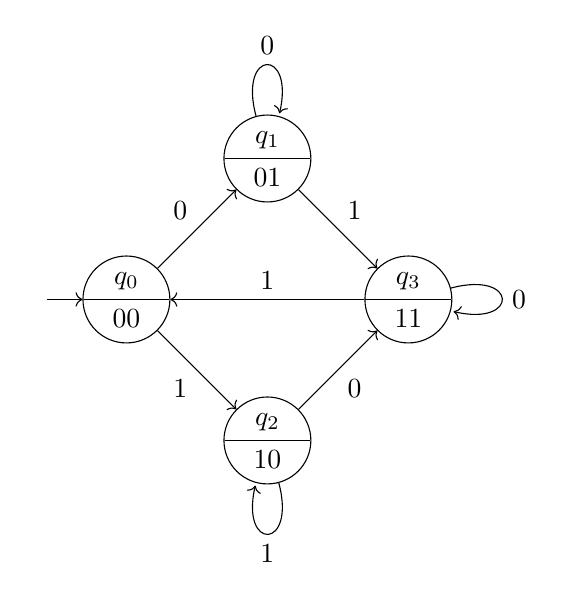
\begin{tikzpicture}[initial text=]
						\node[state with output, initial] (q0) {$q_0$  \nodepart{lower} $00$};
						\node[state with output] (q1) [above right=of q0] {$q_1$  \nodepart{lower} $01$};
						\node[state with output] (q2) [below right=of q0] {$q_2$  \nodepart{lower} $10$};
						\node[state with output] (q3)  [below right=of q1] {$q_3$  \nodepart{lower} $11$};

						\path[->, every node/.style={execute at begin node=$, execute at end node=$}]
						(q0) edge node [above left]  {0} (q1)
						edge node [below left]  {1} (q2)
						(q1) edge node [above right] {1} (q3)
						edge [loop above] node {0} ()
						(q2) edge node [below right] {0} (q3)
						edge [loop below] node {1} ()
						(q3) edge [loop right] node {0} ()
						(q3) edge node [above] {1} (q0);
					\end{tikzpicture}
				}
			\end{center}
		\end{column}
		\begin{column}{0.5\textwidth}
			\begin{center}
				\textbf{Mealy-Automat}\\
				{\scriptsize Ausgabe abhängig von aktuellem Zustand + Eingabe}\\
				\resizebox{!}{0.65\textheight}{
					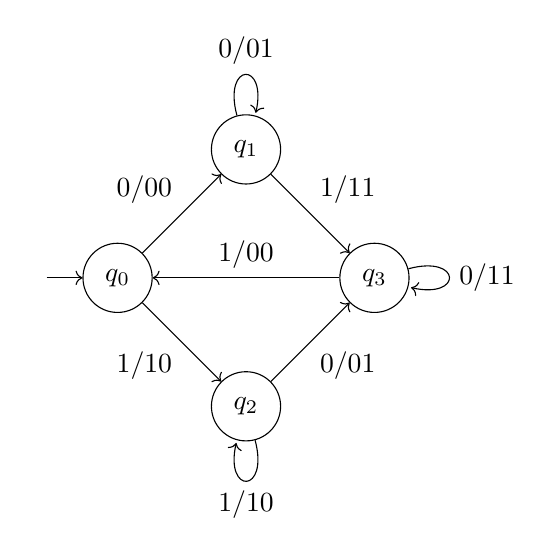
\begin{tikzpicture}[initial text=]
						\node[state, initial] (q0) {$q_0$  \nodepart{lower} $00$};
						\node[state] (q1) [above right=of q0] {$q_1$};
						\node[state] (q2) [below right=of q0] {$q_2$};
						\node[state] (q3)  [below right=of q1] {$q_3$};
						
						\path[->, every node/.style={execute at begin node=$, execute at end node=$}]
						(q0) edge node [above left]  {0/00} (q1)
						edge node [below left]  {1/10} (q2)
						(q1) edge node [above right] {1/11} (q3)
						edge [loop above] node {0/01} ()
						(q2) edge node [below right] {0/01} (q3)
						edge [loop below] node {1/10} ()
						(q3) edge [loop right] node {0/11} ()
						(q3) edge node [above] {1/00} (q0);
					\end{tikzpicture}
				}
			\end{center}
		\end{column}
	\end{columns}
	\begin{center}
		{\scriptsize $I=\{0, 1\}$, $O=\{00, 01, 10, 11\}$, $S=\{q_0, q_1, q_2, q_3\}, \delta, \lambda$ (abh. vom Typen)}
	\end{center}
\end{frame}


\begin{frame}[c, fragile]{RISC-V Multi-Cycle-Prozessor}{}
	\begin{itemize}
		\item Aufteilung einer Instruktion in mehrere Schritte
		\item kürzere kritische Pfade in den einzelnen Teilschritten $\rightarrow$ höhere Taktfrequenz möglich
		\item allerdings benötigt eine Instruktion jetzt auch mehrere Taktzyklen!
		\item komplexeres Steuerwerk, da Zustandsautomat umgesetzt werden muss
	\end{itemize}
\begin{center}
			in der Praxis haben sich Multi-Cycle-Prozessoren nicht durchgesetzt!
\end{center}
\end{frame}

\begin{frame}[c]{RISC-V Multi-Cycle-Prozessor: Schaltbild}{}
	\begin{center}
		\includegraphics[width=0.75\textwidth]{w09_multicycle.png}
	\end{center}
	\centering
	\tiny (Quelle: Vorlesungsmaterialien ERA)
\end{frame}

\begin{frame}[c]{RISC-V Multi-Cycle-Prozessor: Zustandsautomat}{}
	\begin{center}
		\includegraphics[width=0.6\textwidth]{w09_multicycle_states.png}
	\end{center}
	\centering
\end{frame}

\begin{frame}[c]{Feedback}{} 
  \begin{center}
    \includegraphics[width=0.30\textwidth]{\myFeedbackQrFilename}
  \end{center}
  \begin{center}
    \LARGE \href{\myFeedbackLink}{\myFeedbackLink}
  \end{center}
  \vspace{0.5cm}
  \begin{center}
    \small Ein Teil der Folien stammt aus dem Foliensatz von Niklas Ladurner. Vielen Dank dafür!
  \end{center}
\end{frame}

\end{document}